\chapter{Optical Coherence Tomography}

\label{optical_coherence_tomography}
\lhead{\emph{Optical Coherence Tomography}}

Optical Coherence Tomography (OCT) is an important advancement in retinal imaging
technology.  Research leading to OCT technology was made possible during the
1980’s with advancements in the fibre-optics and photonics industries, allowing it to be
developed in 1991 by David Huang and colleagues.\cite{mbib_1,mbib_2,mbib_3} 
Since 1991, many improvements have been made to enable high quality and detailed 
scans of retinal tissues.  The retina, as mentioned previously, is made up of twelve
internal layers with a total thickness between 300-500 $\mu m$.\cite{mbib_4}
These layers are important indicators for monitoring and diagnosing retinal diseases,
which is why opticians use technologies such as OCT to image retinal tissues.

OCT is a non-invasive imaging technique “analogous to ultrasound,” relying on low 
coherence (also referred to as “white light”) interferometry to generate cross-sectional
imagery (or tomography) of retinal tissues within the eye to a “micrometre axial
resolution” of 1-15 micrometres.\cite{mbib_5, mbib_6,mbib_2} Unlike a normal camera,
which only has transverse dimensional resolution, OCT imaging uses low coherence
interferometry to estimate the origin of specific backscatter [from the source of light]
within the retina.\cite{mbib_4}  In other words, OCT images depth as opposed to simply
taking an image of the surface.  Depth resolution can be carried out using three main
methods: Time-domain OCT (TD-OCT), Fourier-domain OCT (FD-OCT) and
Spectral-domain OCT (SD-OCT).  The latter two are normally combined as they are very
similar methods, therefore for simplicity and consistency they will jointly be referred to as
Spectral-domain OCT (SD-OCT).

In the following sections the physics behind OCT technology will be explained further
and the different methods will be described as well as a discussion on image analysis for
different medical diagnostic purposes.

\section{Low Coherence Interferometry}
Because the velocity of light is much larger than that of the
distance between the retinal layers, it is not possible to
directly measure the flight-time of the light returning from the retinal
tissues. \cite{mbib_5} Meaning, the incoming and outgoing light
cannot be differentiated without
the use of low coherence interferometry. Low coherence interferometry
is just as it sounds.  A low coherence light beam, which can be thought
of as a “train of highly autocorrelated overlapping ‘bursts’ of light,”
is directed at a sample surface using an optical probe, which is connected
to the interferometer.\cite{mbib_4}  When the light “burst” hits the
transparent sample, light will be reflected off of the layers within
the sample and its unique autocorrelogram will be detected by its
autocorrelation function to get an idea of the structure of the sample.
\cite{mbib_4,mbib_3,mbib_6} It should be noted that these “bursts” are a
way of explaining what is happening, and are not to be thought of as a
pulsed light source.

In \fref{fig:m_1}, a schematic of the low coherence interferometer used in the classic and current OCT imaging can be found.

\begin{figure}[htbp]
\centering
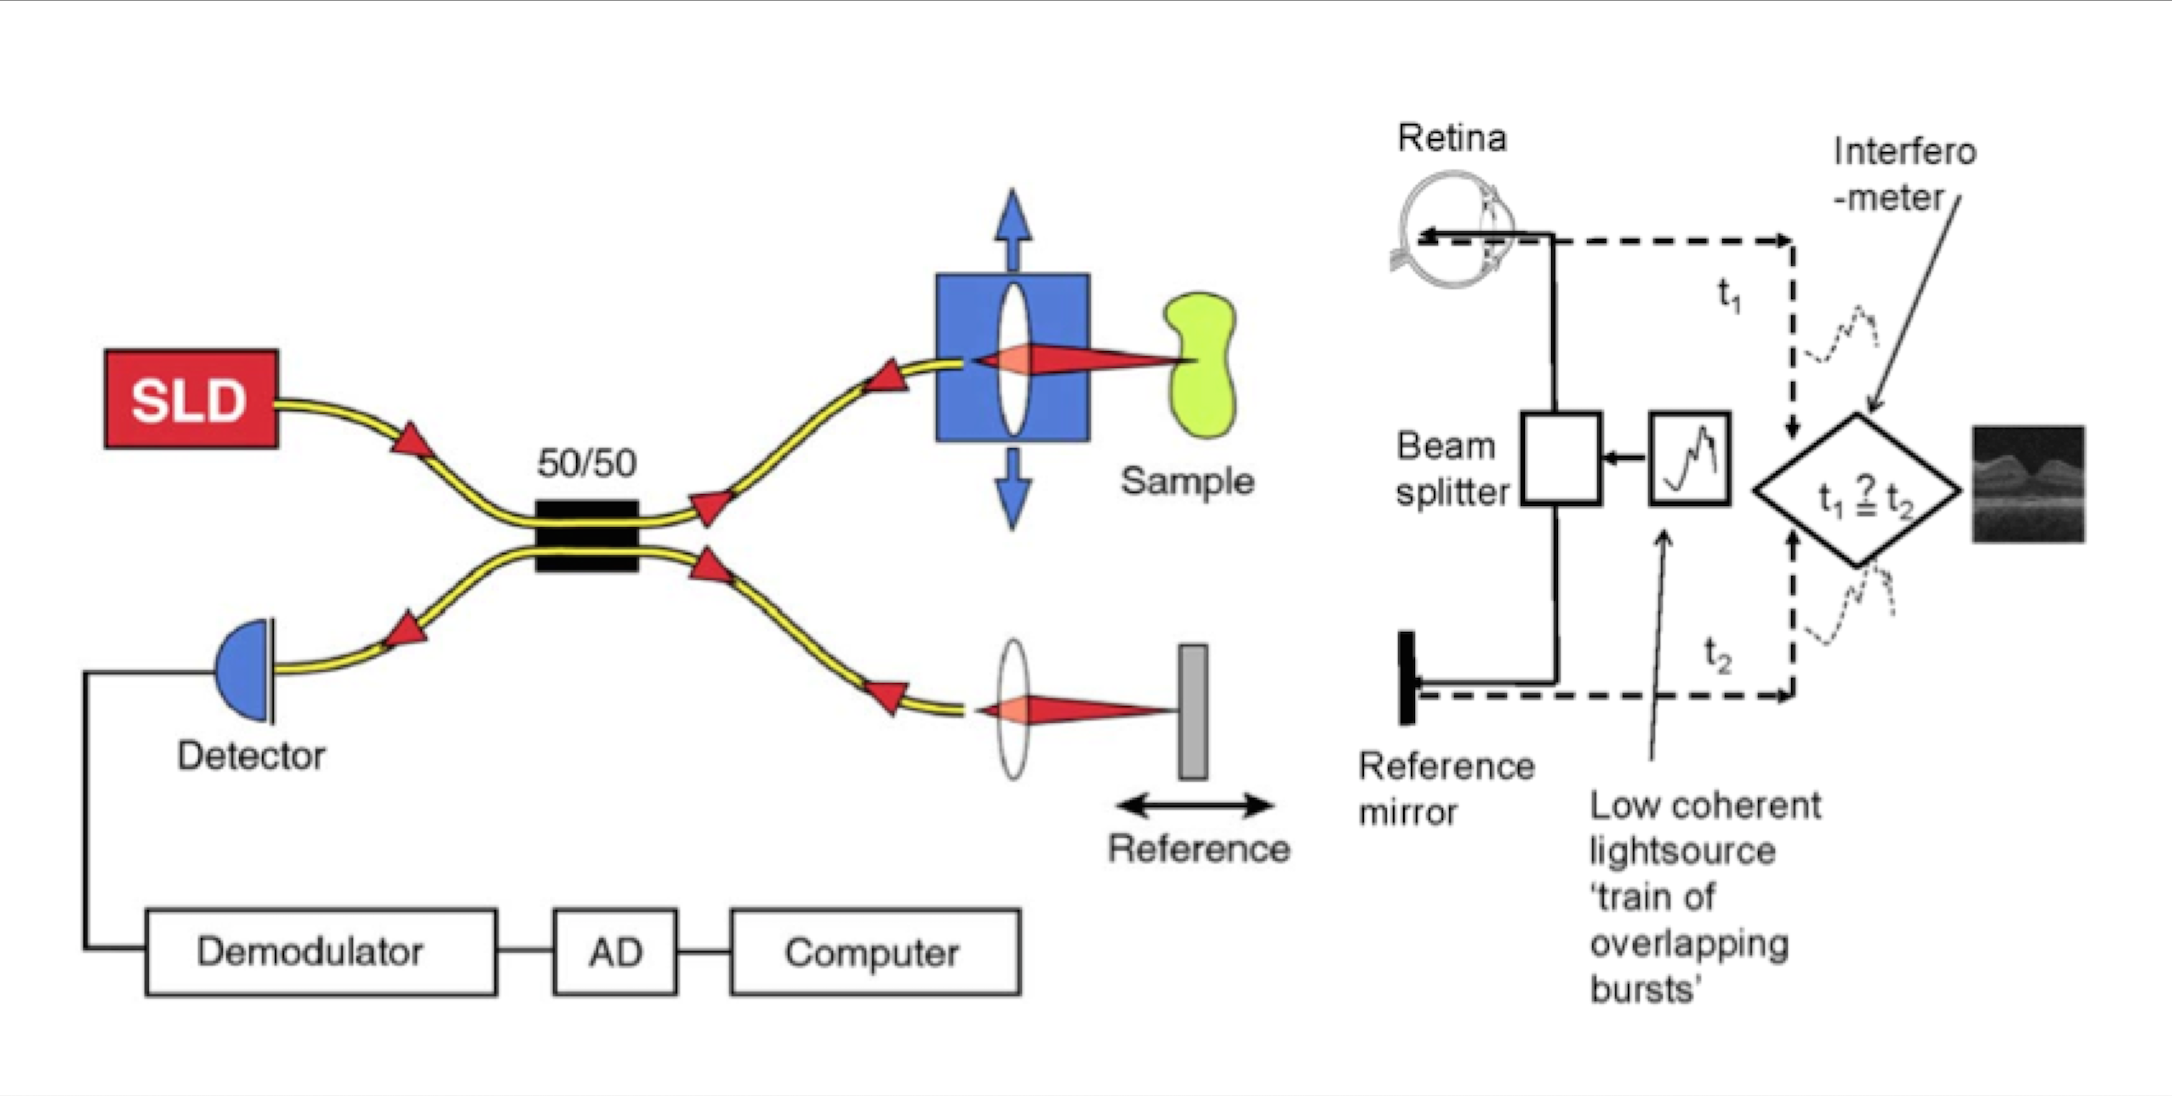
\includegraphics{figures/morgan_1}
\caption{(Left) Classical optical coherence tomography system. 
(Right) A schematic of an optical coherence tomography set-up with particular emphasis on the splitting of light and their interface after being reflected from the retinal tissues as well as from the reference mirror.  An assumption that the time delays of both paths are equal. \cite{mbib_6,mbib_4} }
\label{fig:m_1}
\end{figure}


Super-luminescent LEDs (SLED), also known as super-luminescent diodes (SLD),
which produce wavelengths which reside in the near infrared region, are
traditionally used in OCT interferometry because they are “economical,
compact, long-lasting, and emit high quality beams that couple efficiently
with an optical fibre.” \cite{mbib_6} Also, the amount of light coherence
is inversely proportional to the depth resolution, thus wavelengths longer
than visible light, typically 800–1400nm wavelengths in the near infrared,
are necessary as they penetrate deeper into the retinal tissue layers.\cite{mbib_4,mbib_7}
The resolution of the generated images is limited by the progress of SLD
technology, for example, early systems used SLDs emitting wavelengths around
820 nm, limiting the axial resolution to 11 $\mu m$ in retinal tissues and 15 $\mu m$
in air. \cite{mbib_6}  Today, the CirrusTM HD-OCT device uses SLDs with wavelengths
of approximately 840 nm, and achieve a resolution of 5 $\mu m$ in retinal tissue.\cite{mbib_7}

Inside the interferometer, the light from the SLD is split using a beam splitter.
Other splitting methods such as a 50/50 fibre coupler can be used, but the beam
splitter is the most commonly used method to date.  When the light from the SLD
is split, half of the light is directed to a reference reflective mirror at a
specific distance, while the other is directed into the retinal tissues (sample)
using an optical fibre.  The returning beams from the reference and sample arms
are recombined and produce interference when the distance in the two paths is
equivalent within the coherence length of the light source. \cite{mbib_5,mbib_6}

The interference of two incoming waves can be thought of as the addition of their
respective amplitudes, which is also commonly known in physics as superposition.
When the two waves are in phase, constructive interference occurs and their combined
waveform can be called coherent.  This constructive interference leads to the two
returning waves in the interferometer adding to produce a large interferometric
modulation.  On the other hand, the two returning beams could be largely misaligned
and interfere destructively, with an extreme of them adding up to a flat line.
As the galvanic reference mirror with freedoms in the x and y directions is moved,
the phase of the reference wave changes, and produces a sinusoidal interference
signal, see \fref{fig:m_2}. The summed interference signal forms a wave pulse 
that is converted
from light into an electrical current using a photodetector (light sensor).\cite{mbib_6}
The information is then processed electronically to extract the pulse envelope, which
is then transferred to a computer where it is stored on the memory.\cite{mbib_6}

\begin{figure}[htbp]
\centering
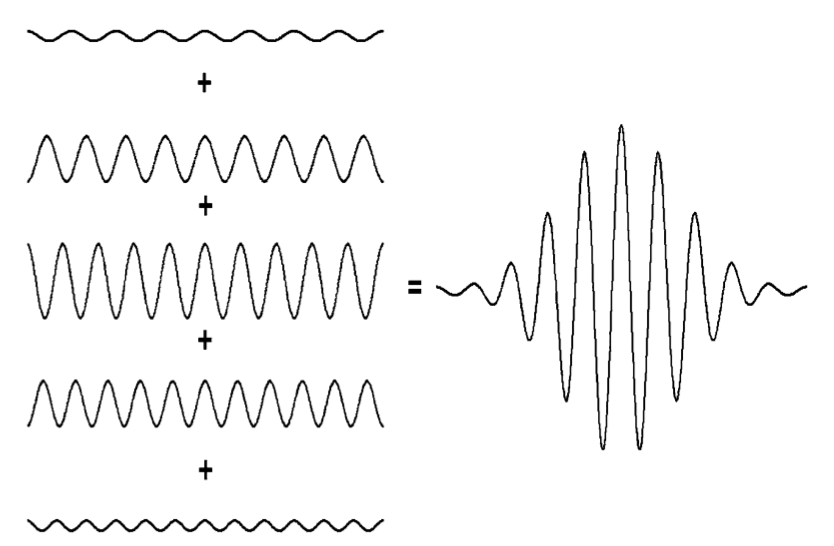
\includegraphics{figures/morgan_2}
\caption{The combined interference signal of a range of wavelengths (left) is 
shown on the right.  The width of this pulse determines the axial resolution of 
the OCT device. \cite{mbib_6} }
\label{fig:m_2}
\end{figure}

The pulse envelope’s width reveals the coherence length by providing
the coherence time (time of flight).  The coherence length can be found
by multiplying the time of flight by the speed of light, and is an
important quantity as it determines the axial resolution of the OCT
device. \cite{mbib_6}  By scanning the retina and recording this
information, a plot of the amplitude against the delay can be generated to
demonstrate tissue reflectivity at successively deeper levels within the
retinal tissue along the axis of beam propagation. \cite{mbib_6}
These scans are known as A-scans.  The A-scans represent the reconstruction
of a plane “through the anterior or posterior segment of the eye.”\cite{mbib_6}
This reconstruction, illustrated in \fref{fig:m_3}, produces a “tomographic
image with an A-scan for each x and y location” and is called a B-scan and is
usually a grey-scale image for diagnostic purposes as the pseudo colour images
make it hard to distinguish details that are easy to miss. \cite{mbib_5,mbib_4,mbib_7}

\begin{figure}[htbp]
\centering
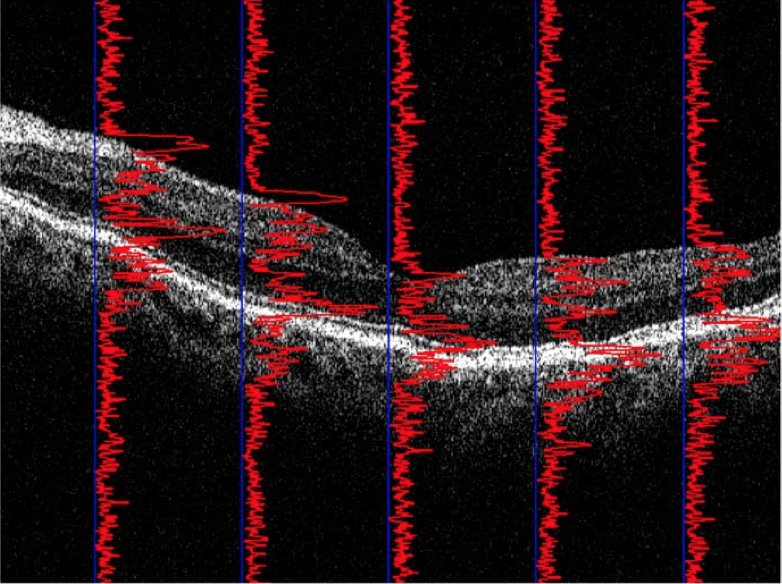
\includegraphics{figures/morgan_3}
\caption{A cross-sectional grey-scale image of the retina, built up from many A-scans which are illustrated as red plot lines. \cite{mbib_6} }
\label{fig:m_3}
\end{figure}


The above description is how Time-domain OCT utilizes low coherence interferometry.
The other option is having a fixed reference mirror and attaching a spectrometer to
the detection arm to record the spectral signal produced by the reflected
 “bursts” of light, which is known as Spectral-domain OCT.\cite{mbib_3} The next
section will go into more detail on the different imaging methodologies.

\section{Time-Domain and Spectral-Domain Optical Coherence Tomography}
Time-domain and Spectral-domain Optical Coherence Tomography differ in the way
the backscatter of the light from the super-luminescent diode from the retinal
tissues is analysed.  To briefly describe the differences between the two main
methods: TD-OCT resolves depth by measuring its flight time through the retina,
whereas SD-OCT uses a spectrometer to measure the difference in wavelength
between the light from the fixed reference arm and that of the light returning
from the retinal tissues to generate these cross-sectional images.\cite{mbib_7}

In both cases, the light wave travels through the retina as illustrated in \fref{fig:m_4} and
is reflected from each layer (detailed image of these layers can also be
found in \fref{fig:m_4} ) because the layers have different refractive indices.
Thus the backscatter of the light from deeper tissues can be differentiated from
backscatter returning from more superficial tissues because it takes longer for
the light to arrive at the sensor; a physical principle utilized in Time-domain OCT
imaging.\cite{mbib_4}

Time-domain OCT is when the reference mirror is mechanically moved to different
positions using the galvanic mirrors with freedoms in the x and y directions,
resulting in a time difference between the light from the reference arm and the
light returning from the retinal tissues.  These time differences depend on the
depth at which the light is backscattered from and can be used to reconstruct
retinal structure.  Since the speed at which the mirrors can be moved is limited
mechanically, only thousands of A-scans can be generated per second.” \cite{mbib_4}

\begin{figure}[htbp]
\centering
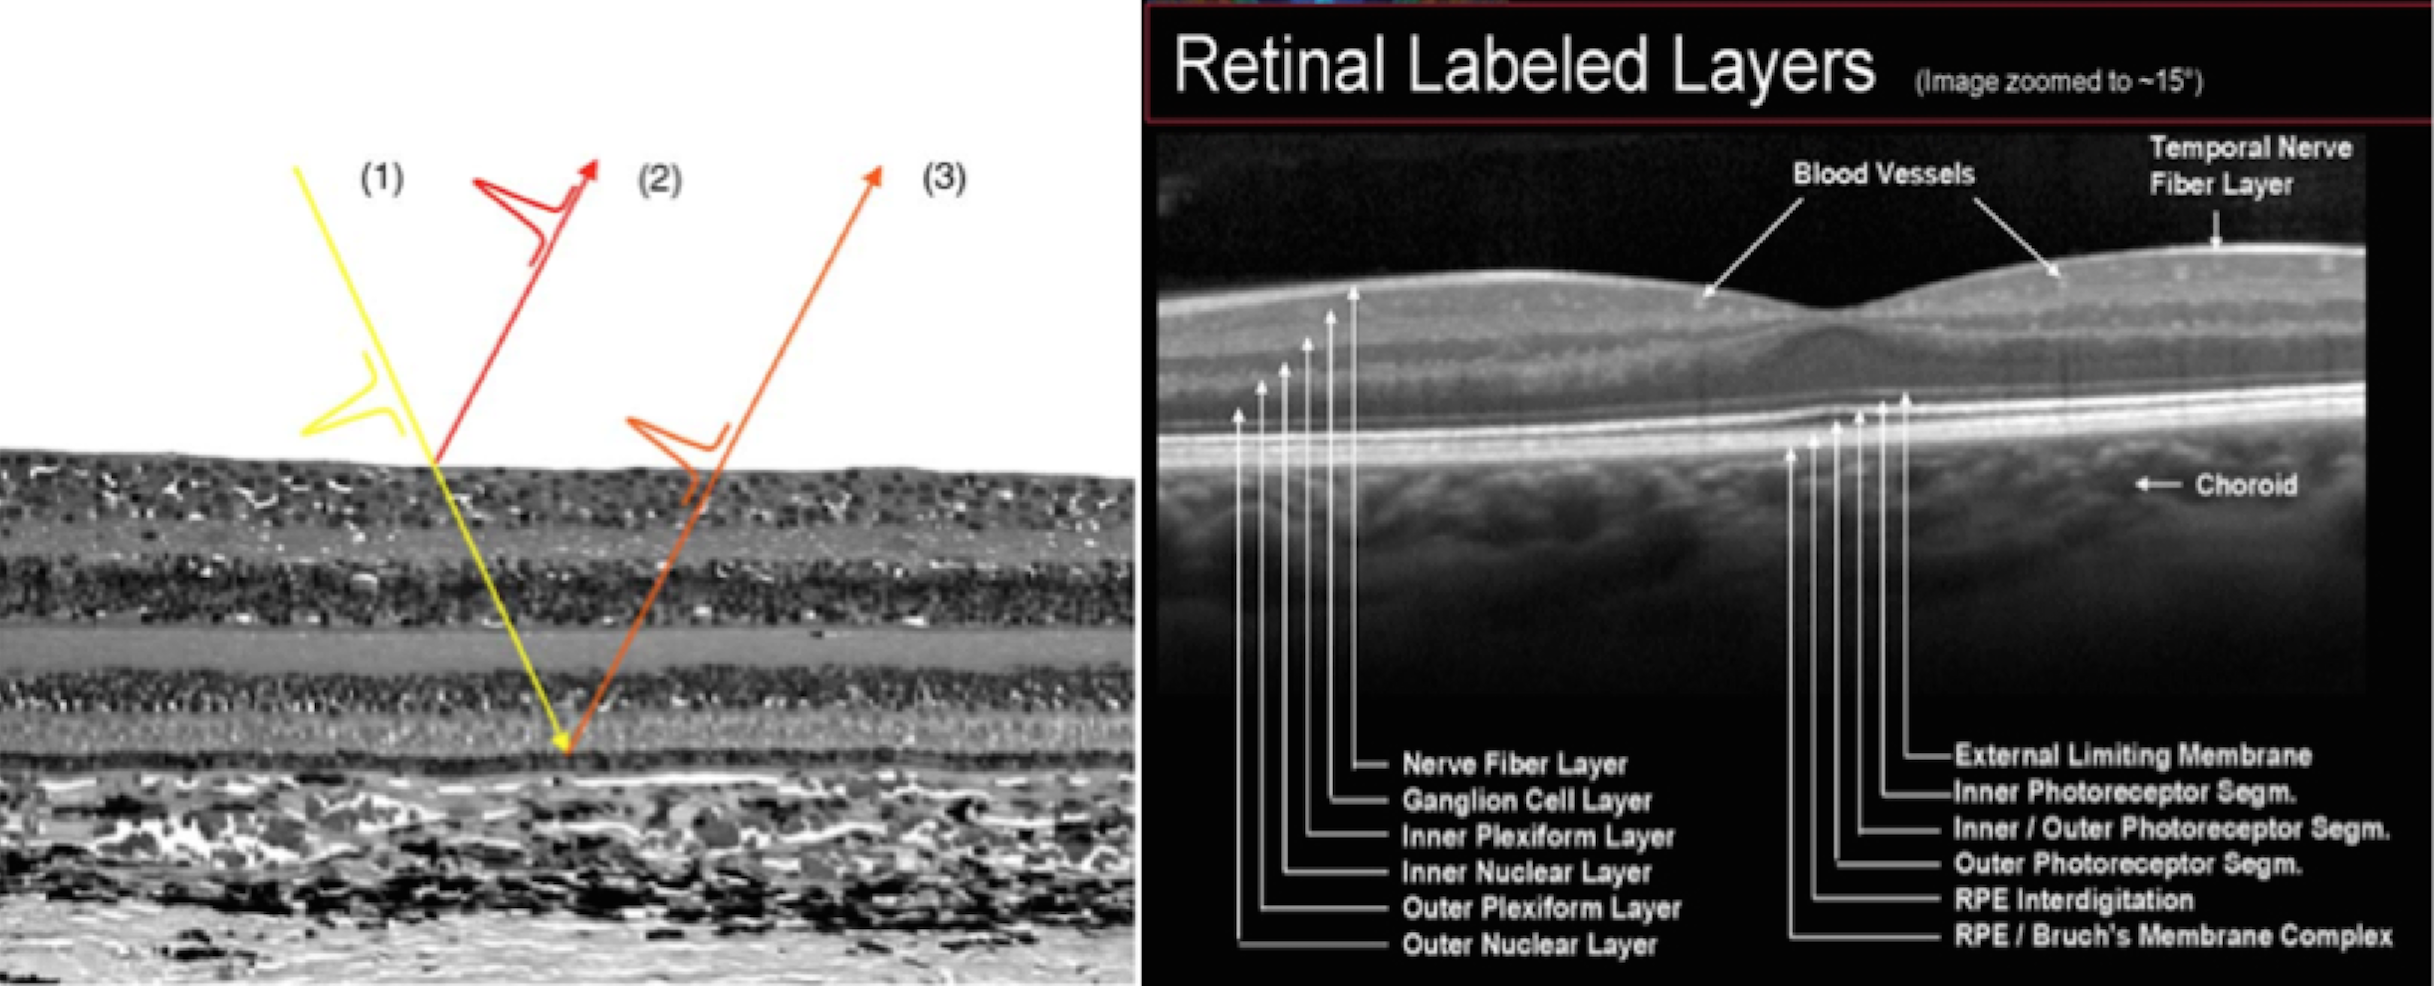
\includegraphics{figures/morgan_4}
\caption{(Left) "The optical coherence tomography beam is scanned across the retina (1).
The delay of a superficial reflection (2) is shorter than that of a deeper reflection (3)" (Right) A two dimensional black and white SD-OCT scan with an image zoom of 15$^\circ$.\cite{mbib_6}  This scan shows the retina with retinal
tissue layers labelled using arrows to give meaning to the image.\cite{mbib_8} }
\label{fig:m_4}
\end{figure}

Another physical principle that is utilized in Spectral-domain OCT imaging is the
fact that the reflected light will have a different spectral fingerprint than the
initial light sent into the eye which will return from the reference arm.  Instead
of continuously moving the reference arm, as in TD-OCT, the reference arm is kept
fixed.

The main difference between Fourier-domain and Spectral-domain OCT is that in
FD-OCT the SLD’s light is rapidly modulated over its centre wavelength providing
another tag to the light; whereas in SD-OCT a broadband light source is used,
and the signal from the interferometer is spectrally decomposed using a diffraction
grating and a CMOS (Complimentary Metal Oxide Semiconductor) or CCD
Charge Coupled Device) linear sensor.\cite{mbib_4}
Thus a spectrometer is used to detect the spectrum created by the backscatter
to produce an image of the retina.  Once the signal is obtained a Fourier transform
(a mathematical procedure which extracts the frequency spectrum of a signal) is
applied to the spectral signal to determine the depth of all resultant scatters from
the tissues at the x and y coordinates.\cite{mbib_4,mbib_9} SD-OCT technology
proves to be more advanced than original TD-OCT in that it provides greater
resolving power of the retinal layers, significantly higher scan density, and faster
data acquisition. \cite{mbib_2}

\section{Images}
A-scans and B-scans were mentioned previously at the end of the low
coherence interferometry section.  For many years two dimensional B-scans were
the highest achievable image possible because OCT technology could not take
images fast enough to acquire enough images to construct a three dimensional
image of the retina.  Due to patient comfort, and safety requirements limiting how
much light can be projected onto the retina, images can only be taken for 1-3 seconds. \cite{mbib_4} With the improvement of SD-OCT, hundreds of thousands
of A-scans can be taken a second as opposed to the 400 A-scans a second achieved by
commercially available TD-OCT machines; making three dimensional images of the retina
possible.\cite{mbib_4}  Three dimensional images are now widely used in the clinical
setting as a standard of care.  As the technology improves, increasing the number of
A-scans taken in a second, higher resolution can be achieved in 3-D image volumes.\cite{mbib_4}  \fref{fig:m_9} illustrates the difference between the two 
and three dimensional images.

\begin{figure}[htbp]
\centering
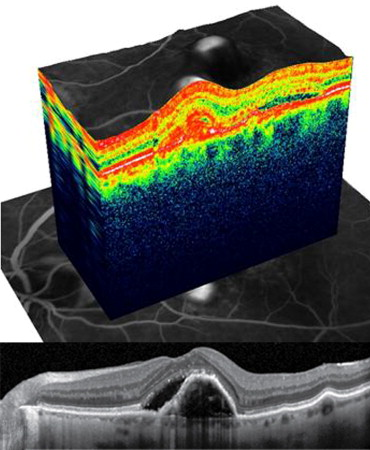
\includegraphics{figures/morgan_9}
\caption{ Overlay of the different retinal image scans using optical coherence tomography. The top image is a three dimensional image of the retinal with a fundus image below, and the bottom image is a two dimensional B-scan of the same retina which was used with a series of B-scans to produce the three dimensional image appearing above. \cite{mbib_13} }
\label{fig:m_9}
\end{figure}

The overall resolution of these images in the x and y directions is dependent on the
speed and quality of the galvanic mirrors used in TD-OCT.  In the z direction the
coherence of the light limits the resolution.  Both of these limitations were mentioned
previously in the section describing the methods of analysing the returning light
backscatter from the eye.

Ultimately OCT imaging technology is looking for a way to achieve isotropic images
of the retina, meaning the size of each element imaged is the same in all three
dimensions.  OCT devices commercially available currently can only achieve images
isotropic in the x-y plane, and have pixel volume sizes
of 30 × 30 × 2 $\mu m$. \cite{mbib_4}
This is because current OCT technology always has higher resolution of depth than
in the x-y plane. \cite{mbib_4}  Although a completely isotropic image is not possible
with current technology, there is an advantage to having “x−y isotropic imaging”.\cite{mbib_4} This method reduces the number of assumptions that 
have to be made when combining different retinal tissue sample
images, and allows the properties of the retina to be readily quantified for medical purposes.\cite{mbib_4} This helps ophthalmologists add more accurate images to the collection of information
making up retinal morphology.

Although the images are of high quality and resolution, the practitioner must consider
some other limitations.  For example corneal conditions such as dry eye, blinking, and
dilation of the eyes.  To tackle these limitations: dry eye can be addressed by applying
artificial tears to the patient’s eyes prior to the examination; blinking can be prevented
by shortening the scanning time and having the patient focus on the stimulus (which appears as a cross of green segments similar to that of a star); and in order to
achieve a larger scan of the retina, many practitioners dilate the patients eyes as
in many other retinal imaging examinations.\cite{mbib_4}

\section{Medical Applications of OCT}
OCT has many biomedical applications, however, the chief among them is retinal imaging and is particularly useful for monitoring, identifying, and quantitatively
assessing retinal diseases.\cite{mbib_9,mbib_4, mbib_5}  Before OCT there was
very little information in the database of retinal morphology.  With OCT imaging
this database has grown, providing a wealth of new information and has enabled
practitioners to closely  monitor retinal diseases and help guide them in the treatment
of patients with existing problems for therapeutic purposes.\cite{mbib_4}

OCT imaging currently used widely to determine the extent and amount of
retinal thickening to help guide these treatments prior to operation, as well as postoperative 
monitoring to ensure the patient is healing as expected.
This is done by imaging the thickness of the retinal tissue layers to find areas where a
retinal layer is thicker than the rest of that layer in the rest of the retina.  Retinal
layer thickness is the most common property currently utilized by medical professionals
in the tracking and diagnosing of retinal diseases, however, other properties can be looked
into such as analysing the images for textural properties in each of the layers, and quantifying
fluid parameters. \cite{mbib_4}

\subsection{Diabetic Macular Edema (DME)}
The most common application is in diabetic macular edema (DME). A patient with DME  leaks
fluid in the macula which in turn causes visual loss in said patient.  An original research
paper titled Early Treatment in Diabetic Retinopathy Study demonstrates that early treatment
of patients with DME with a focal laser can prevent further visual loss when targeting the
thickened areas of the retina. \cite{mbib_4}  This is done by analysing the thickness of the
retina and determining if there is an area of a retinal layer that is thicker than the rest.
An example of an OCT scan of someone with DME can be found in \fref{fig:m_5}.

\begin{figure}[htbp]
\centering
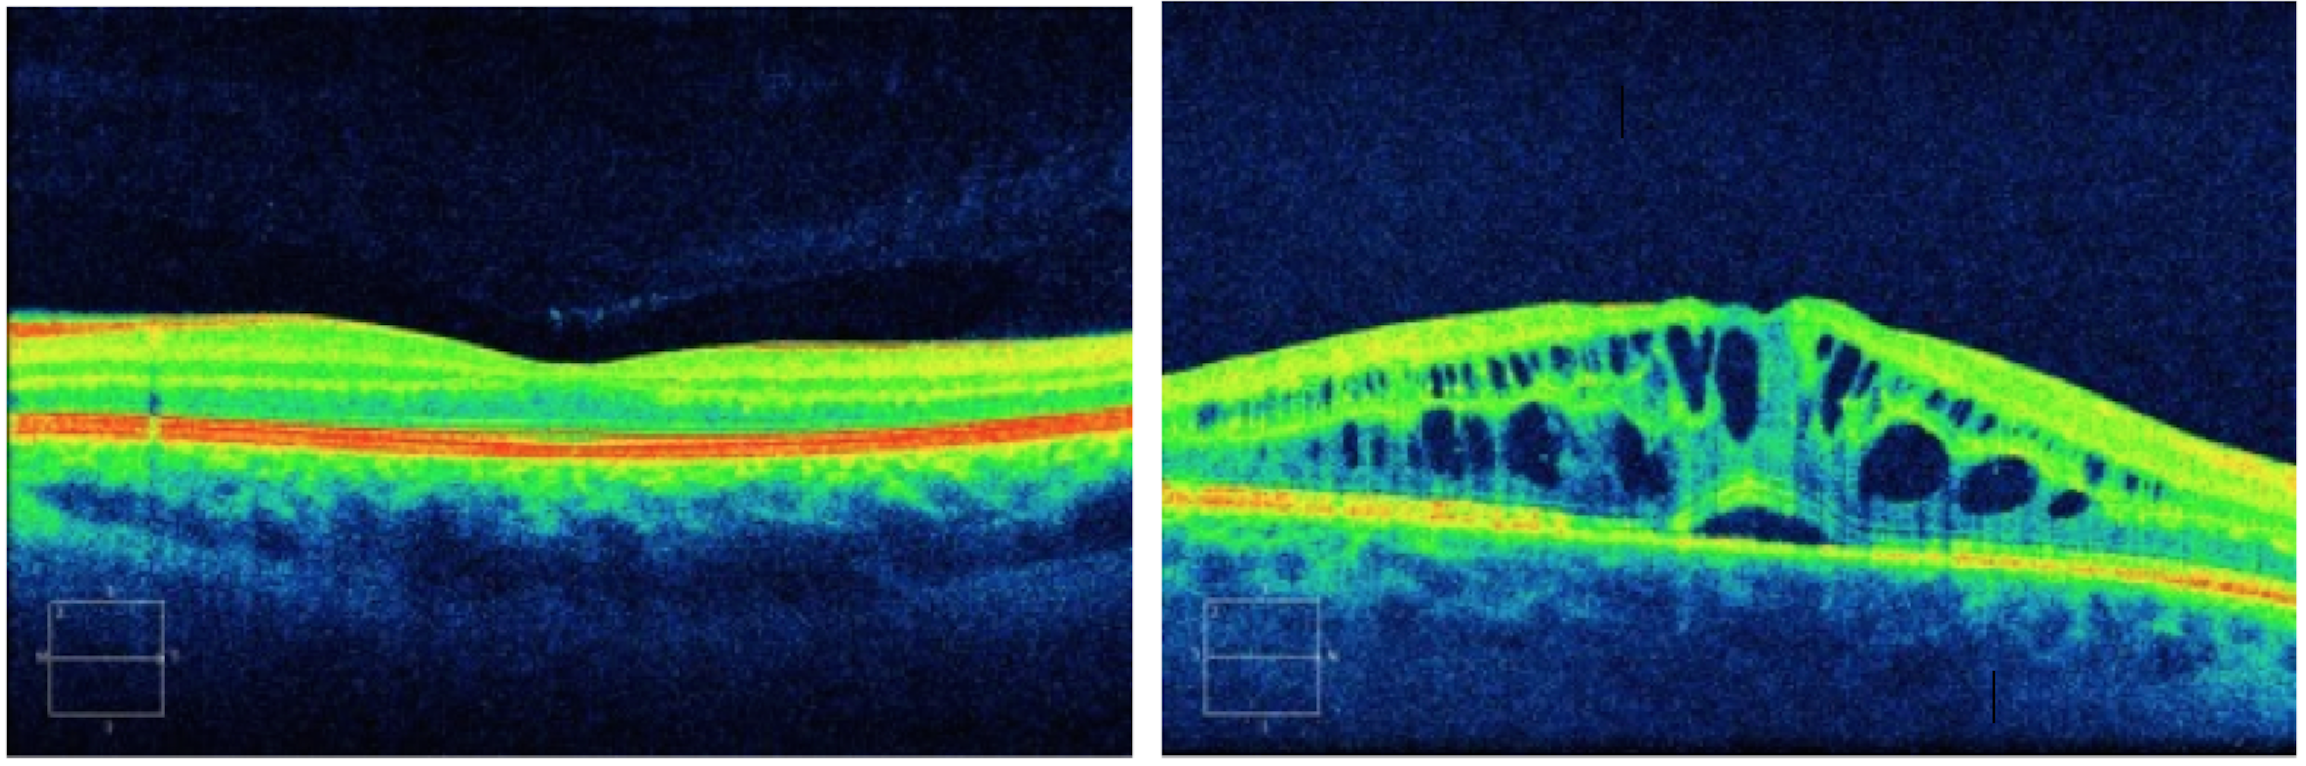
\includegraphics{figures/morgan_5}
\caption{Two images appear in this figure.  The left is an image demonstrating a patient with a normal retinal OCT scan in pseudo colours, while the left is that of a patient suffering from DME. \cite{mbib_10} }
\label{fig:m_5}
\end{figure}

\subsection{Glaucoma}
Glaucoma is a disease which causes gradual damage to the optic nerve.  
As mentioned in \cref{anatomy}, the result of this damage is visual field 
loss. \cite{mbib_6} If diagnosed early, this 
disease can be treated to reduce the risks of vision loss by using OCT 
images to observe thinning in the retinal nerve fiber layer and ganglion cell 
layer.  Both layers are extremely useful in the treatment and management 
of glaucoma as they serve as indicators of the extent of the optic nerve 
damage. \cite{mbib_4}
Since the optic nerve is where glaucoma manifests, the optic nerve head 
is another structure important to the study of glaucoma. \cite{mbib_4}
Along with thickness analysis, texture analysis can also be useful in the 
care for patients with glaucoma.  Texture analysis is possible by utilizing 
the local variations in brightness within one small area of an 
image. \cite{mbib_12} \Fref{fig:m_6} is an image of example optic nerve 
OCT image analysis and compares the different methods of analysing 
the images.

\begin{figure}[htbp]
\centering
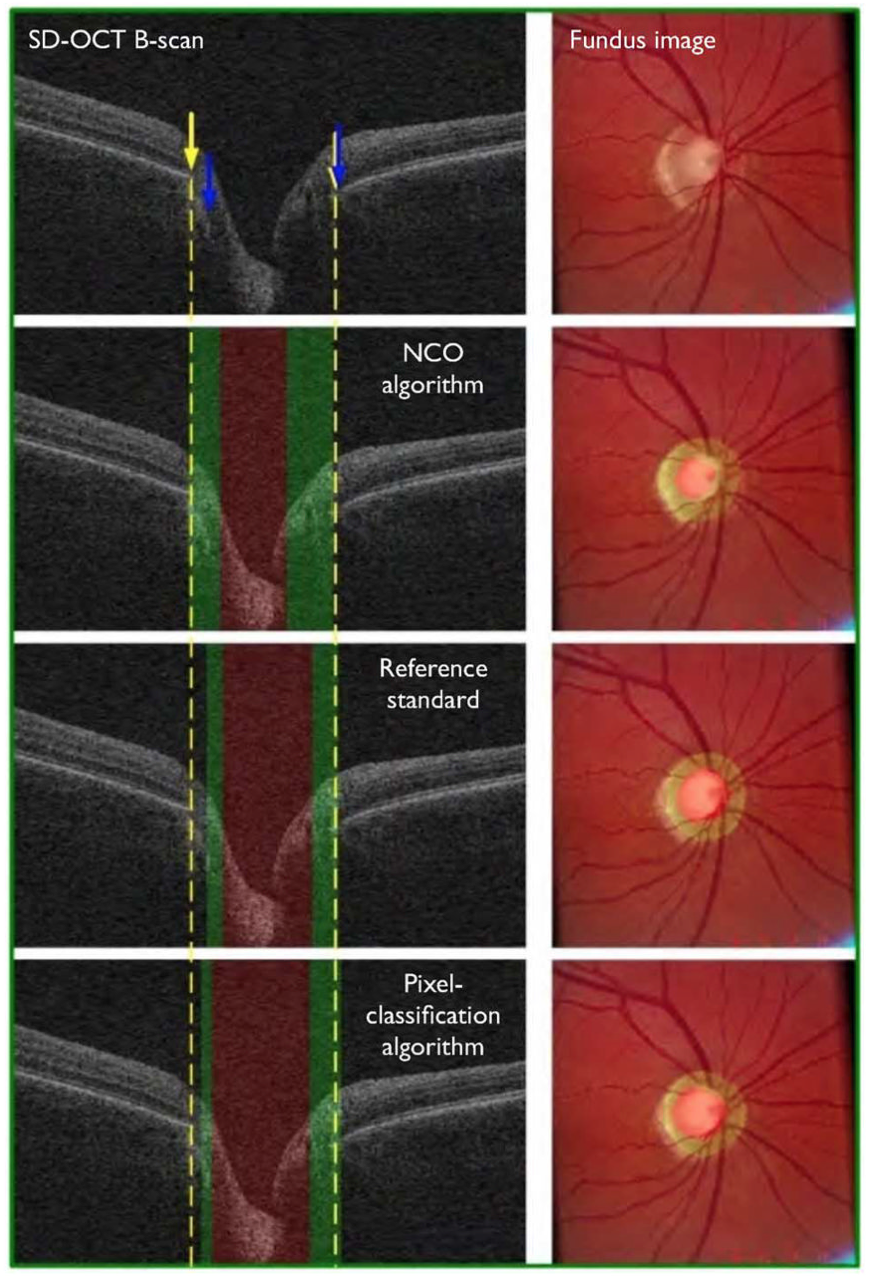
\includegraphics{figures/morgan_6}
\caption{This figure includes from top to bottom: a raw SD- OCT B-scan and corresponding
fundus image (top), structure-based (row 2), expert on fundus photography (row 3) and
pixel-classification-based (bottom) segmentations overlapping with raw SD-OCT and
corresponding fundus image.  From left to right: SD-OCT central B- scan (left) and
fundus image (right).  Yellow arrows indicate the position of the neural canal opening
(NCO) from algorithm (with dashed yellow line indicating projected NCO position).
Blue arrows indicate clinical disc margin from RS. Green and red colours indicate each
method’s projected rim and cup regions, respectively. \cite{mbib_4} }
\label{fig:m_6}
\end{figure}

\subsection{Symptomatic Exudate-Associated Derangements (SEADs)}
Another application of texture analysis is using textural properties along with
layer-based properties to detect retinal lesions in both two and three dimensional
OCT images. Out of all of the different types of lesions, symptomatic exudate-associated derangements (SEADs) are the prime interest of
experts assessing the severity of diseases such as age-related macular degeneration and diabetic macular edema.  SEADs are detected in a two step process when analysing OCT images.  First, possible candidates are identified in the OCT scans after the retinal layers are segmented (a process by which the different layers are separated from each other in the image) and the image is then flattened (when the curve of the layers due to the curve of the retina is flattened).  Once flattened, the area is then analysed to determine whether or not the candidate is a SEAD or not. 
\cite{mbib_4} Examples of these can be found in \fref{fig:m_7}

\begin{figure}[htbp]
\centering
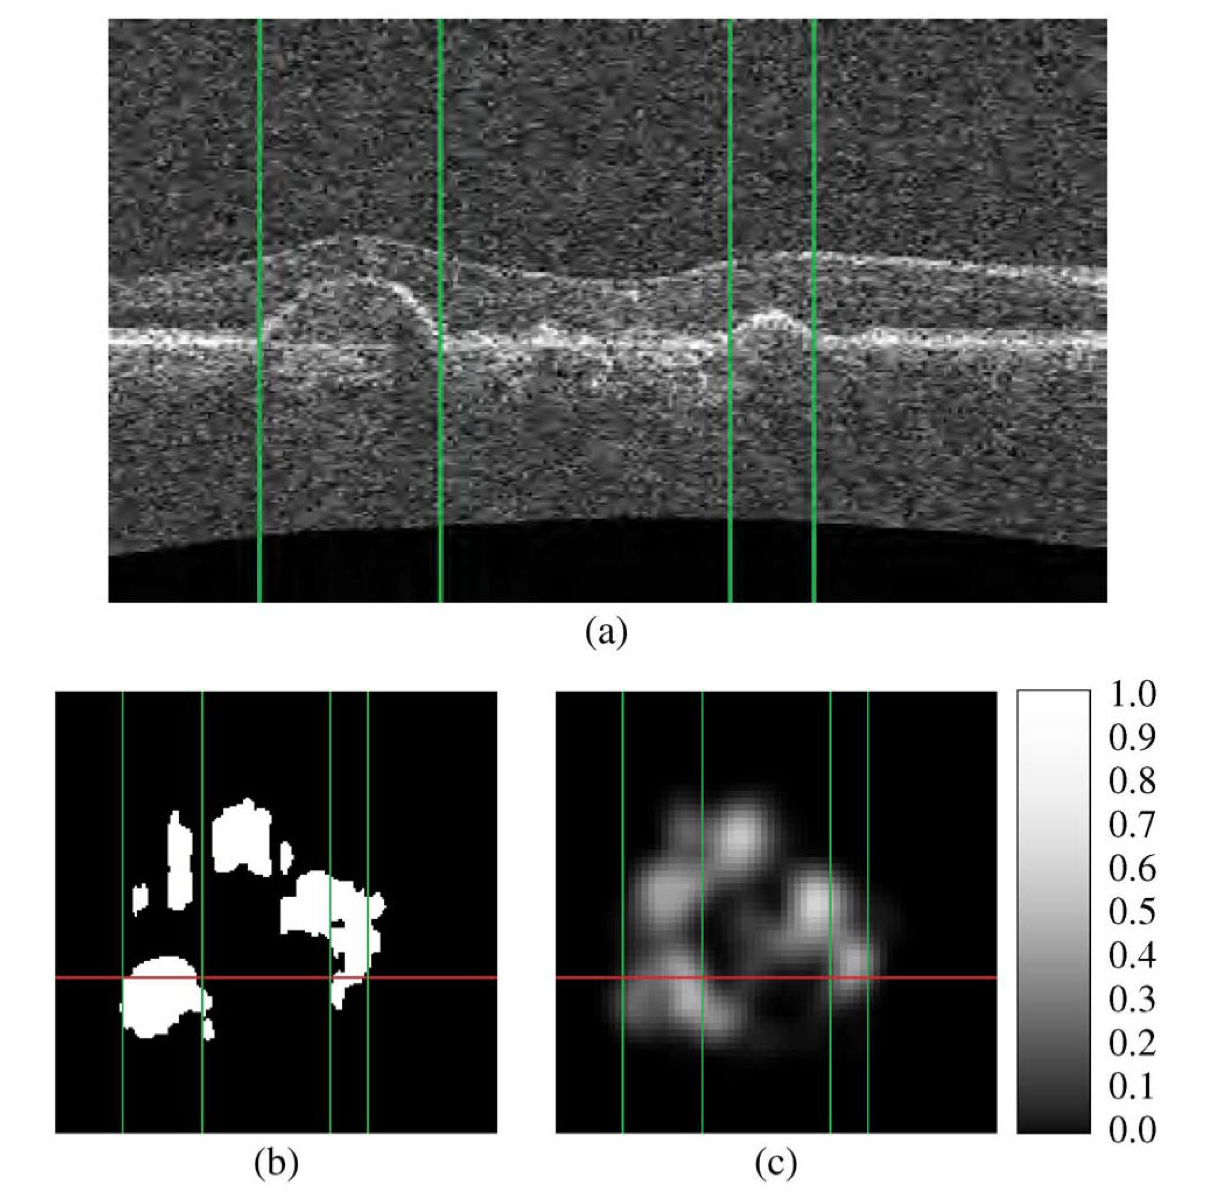
\includegraphics{figures/morgan_7}
\caption{SEAD footprint detection: (a) is an x-z slice running through the SEADs in SD-OCT volume; (b) and (c) are SEAD probability maps in x-y generated automatically using expert standards.  Note the probability scale in panel (c). Projection of the x − z slice in x − y plane is represented by a vertical line in (b) and (c). The location of the SEADs which are visible in panel (a), are indicated by vertical lines in each panel. \cite{mbib_4} }
\label{fig:m_7}
\end{figure}

\subsection{Choroidal Neovascularization}
Choroidal neovascularization is another blinding disease clinically known as the wet form of macular degeneration due to age.  The main indicators of this disease are outer and sub-retinal fluid. \cite{mbib_4}  By using OCT imaging to quantify fluid parameters and affected retinal tissues in patients with this disease, proper treatment can be applied.\cite{mbib_4} \fref{fig:m_8} is contains an OCT scan of someone suffering from choroidal neovascularization.

\begin{figure}[htbp]
\centering
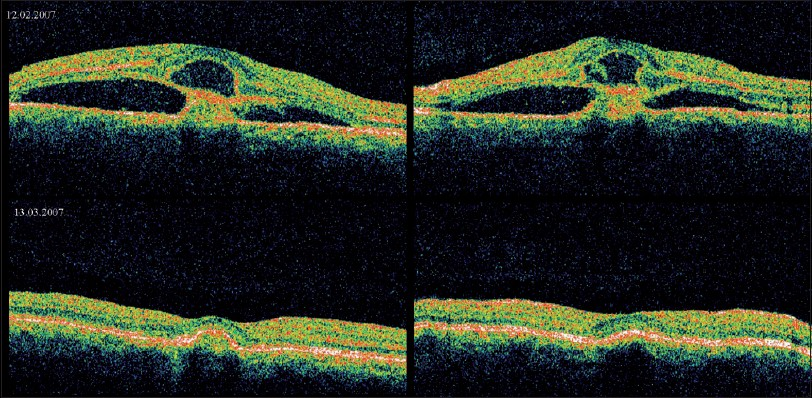
\includegraphics{figures/morgan_8}
\caption{ Optical coherence tomography images show a sub-foveal choroidal neovascular membrane associated with sub-retinal fluid and cystoid macular edema at baseline (first row) and below are one month follow-up optical coherence tomography scans which show the disappearance of cystoid edema and complete resolution of sub-retinal fluid post treatment. \cite{mbib_11} }
\label{fig:m_8}
\end{figure}

\section{Further Improvements}
The current state of OCT technology can already achieve much better images
 of the retina than the original technology developed in 1991.  Previously 
unachievable capabilities of these machines are now clinically standard practice 
in the medical diagnosis of several retinal diseases.  Although these
 improvements are highly effective in improving the technology for retinal 
imaging, further research can be done to obtain images of deeper structures 
within the eye such as the choroidal vessels, which are a structure in the optic 
nerve and relevant to the study of damage caused by glaucoma. \cite{mbib_4} 
Current commercially available machines use wavelengths around 840 nm
and only allow medical professionals to image the retina.  Longer wavelengths 
around 1000-1300 nm would enable the OCT imaging light to penetrate deeper 
into the tissue and image deeper structures such as choroidal vessels. 
\cite{mbib_4}  However, at these increased wavelengths, the limits of CCD 
(Charge Coupled Device) technologies are encountered.  These detectors 
were briefly mentioned when discussing the differences between Spectral 
and Fourier Domain methodologies, but the actual technology was not 
described. 
 
CCDs are highly sensitive photon detectors, conventionally made using 
silicon, which are divided into a large number of light-sensitive pixels.  These 
pixels are used to build up an image of the retina by converting the light 
incident on the silicon detector into one or more electrons that are collected 
as seen in \fref{fig:CCD} and stored in the potential well created by the incoming 
photons. The number of electrons displaced is directly proportional to the 
intensity of the incident light at each pixel.

\begin{figure}[htbp]
\centering
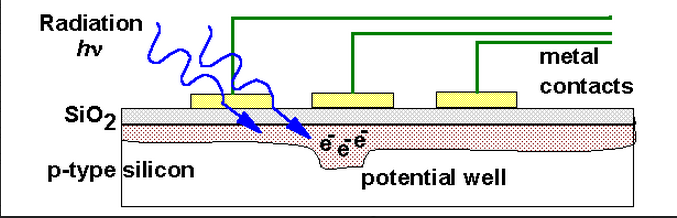
\includegraphics{figures/CCDSchem}
\caption{Illustration of the functionality of a CCD.  Incoming radiation is incident on the CCD and one or more electrons are displaced and collected to determine the intensity of the light at each pixel. \cite{poo1} }
\label{fig:CCD}
\end{figure}

CCDs are sensitive to a wide wavelength range ranging from 400 -1050 nm 
with a peak sensitivity around 700 nm. The lack of sensitivity at long wavelengths
has affected the widespread adoption of these devices. \cite{poo2} 
 
If the amount of energy of the incoming photon is too small, the detectors are 
not able to register the incident light. This is due the physical principle that by
increasing the wavelength of the imaging light, the energy of the photon hitting
the CCD detector decreases, and if the energy is not large enough for the
detector to register, the silicon CCD is no longer the appropriate photodetector. 
In a long wavelength OCT cheap silicon detectors have been replaced by 
InGaAs detectors, which are sensitive between 800-1700 nm.

